\section{What the averaged criteria do and do not permit}

\subsection{The cubic normalization and the precise new target}

For clarity, here is the full normalization used in the application.
Let $H$ be the splitting field of $X^3-X-1$. This is the Hilbert
class field of $K=\Q(\sqrt{-23})$, whose class group has order $3$.
If $\psi$ is a nontrivial ideal-class character of $K$ and
$F=\Q(\theta)$ for a root $\theta$, then
\[
 \zeta_F(s)=\zeta(s)L_K(s,\psi),\qquad
 \zeta_H(s)=\zeta(s)L(s,\chi_{-23})L_K(s,\psi)^2.
\]
These are the exact factorization identities established and referenced
in the predecessor's cubic benchmark \cite{priorcubic}.
The degree-two factor is a Hecke function over $K$; it is not a
Dirichlet $L$-function over $\Q$.

Define the normalized Euler--Kronecker constant by
\[
 \zeta_H(s)=\frac{\kappa_H}{s-1}
              +\kappa_H\gamma_H+O(s-1).
\]
If $-\zeta_H'/\zeta_H=\sum a_H(n)n^{-s}$, its coefficients obey
$0\le a_H(n)\le6\Lambda(n)$ and
\[
 a_H(n)=3\!\!\sum_{\substack{N\mathfrak a=n\\{}[\mathfrak a]=1}}
                 \Lambda_K(\mathfrak a).
\]
The identity follows by summing the three class characters; character
orthogonality keeps exactly the principal ideal powers. Thus the
statistic in the previous section is also
\[
 \mathcal R_H(x)=
 \sum_{n\le x}a_H(n)\left(\frac1n-\frac1x\right)
       -\log x+\gamma_H+1.
\]

Writing $z=s-1$, direct multiplication gives
\[
 \frac{-\zeta_H'(s)/\zeta_H(s)}{s(s-1)}
   =z^{-2}-(\gamma_H+1)z^{-1}+O(1).
\]
This verifies both subtractions at $s=1$.
At a zero $\rho$ of multiplicity $m_\rho$, the residue is
$m_\rho/[\rho(1-\rho)]$. On the real part of the critical strip it
is positive; beyond $1$ there are no zeros. Therefore the
positive-part and moving-average theorems apply without a
zero-avoiding auxiliary analytic twist.

There are now three concrete targets, each sufficient:
\[
\boxed{\begin{aligned}
 &\int_X^{2X}(\mathcal R_H)_+\,dx
        \ll_\varepsilon X^{1/2+\varepsilon}
        &&\text{on dyadic }X;\\
 &\int_X^{2X}(\mathcal R_H)_+^2\,dx
        \ll_\varepsilon X^\varepsilon
        &&\text{on dyadic }X;\\
 &\int_X^{2X}\mathcal R_H\,dx
        \le C_\varepsilon X^{1/2+\varepsilon}
        &&\text{for all large real }X.
\end{aligned}}
\]
Every statement is for all $\varepsilon>0$. The third is genuinely
one-sided; replacing its inequality by absolute-value big-$O$
notation would unnecessarily strengthen it.

None is proved arithmetically here. A successful estimate would
settle a nonabelian RH instance, and would do so using information
beyond the source's Dirichlet factors. Conversely, this fixed field's
RH supplies conventional smoothed error bounds and hence these
averaged bounds. The distinction is a weaker \emph{form of control
to aim for}, not a claim of a conjecture logically weaker than that
RH instance.

For this statistic, the elementary bound
$|\mathcal R_H(x)|=O_H(\log^2(2x))$ also means that integer starting
points suffice for the third target: changing $X$ by at most one
changes the two endpoints by bounded amounts and costs only
$O_H(\log^2(2X))$ in the unnormalized integral. This observation
does not permit exponentially sparse starting points.

\subsection{A continuous example separating average and pointwise control}

The relaxation remains real even if a function tends to zero and
varies slowly. For each $X=2^k$, put a triangular bump at $3X/2$,
of height $X^{-1/4}$ and half-width $X^{3/4}/4$, and set $R$ to
zero between these bumps. The supports are disjoint and lie within
their respective dyadic bins. Exact triangle areas give
\[
 \int_X^{2X}R(x)_+\,dx=\frac14X^{1/2},
 \qquad |R'(x)|\le\frac7x
 \quad\text{where the derivative exists}.
\]
The function is continuous and tends to zero. Its Mellin integral
converges absolutely, and defines a holomorphic function, throughout
$\Re s>1/2$. Nevertheless, at the bump centers,
\[
 R(3X/2)=X^{-1/4},
\]
which is not $O(x^{-1/2+\varepsilon})$ for any
$0<\varepsilon<1/4$. Thus the positive-part mean criterion does
not hide an equivalent pointwise assumption on general functions.

\begin{figure}[htbp]
\centering
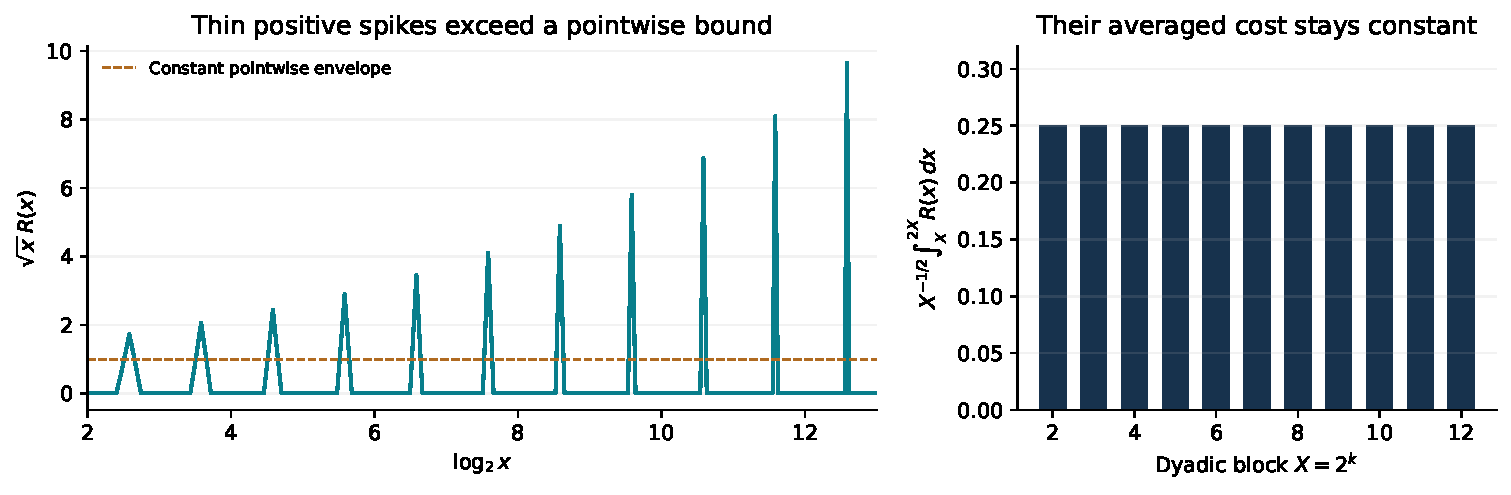
\includegraphics[width=\linewidth]{figures/averaged_spikes.pdf}
\caption{A synthetic exact model, not prime data. The normalized
pointwise peaks grow, while every normalized dyadic positive area is
$1/4$. The mathematical identities are checked with rational
arithmetic; floating point is used only to draw the figure.}
\end{figure}

\subsection{Two further analytic checks}

\textbf{The sign and real-pole hypothesis cannot be omitted.}
For $\beta<a<1$, the function $R(x)=-x^{a-1}$ has
$R_+=0$, yet $F(s)=-1/(s-a)$ has a real pole of negative residue.
Likewise $R(x)=-x^{a-1}\log x$ gives
$F(s)=-1/(s-a)^2$: its residue is zero, but it has a double real
pole. In fact the theorem needs simplicity only at real poles;
nonreal poles may have arbitrary finite order.

\textbf{A positive averaging kernel can still conceal poles.}
It is essential that the moving-box multiplier has no zeros in
the desired half-plane. Set
\[
 R(x)=x^{a-1}\cos\!\left(\frac{\pi\log x}{\log2}\right),
 \qquad \beta<a<1.
\]
Then the positive weighted combination
\[
 R(x)+2^{1-a}R(2x)=0
\]
vanishes identically, while the Mellin transform of $R$ has poles
at $a\pm i\pi/\log2$. Positivity of averaging weights alone is
insufficient. The explicit zero-free multiplier
$(h^s-1)/s$ is what makes the moving-box theorem valid.

There is also a useful weighted-box variant. For real $\nu$, set
\[
 T_{h,\nu}R(x)=x^{-1-\nu}\int_x^{hx}t^\nu R(t)\,dt.
\]
The same calculation yields multiplier
$(h^{s+\nu}-1)/(s+\nu)$, whose zeros lie on
$\Re s=-\nu$. Thus the moving criterion remains valid on
$\Re s>\beta$ whenever $\beta+\nu\ge0$. This can accommodate
a power normalization arising naturally from an averaged
determinant calculation. For an arbitrary varying weight, the
transform must be checked afresh.
